\section{Mehrfache Integrale \formelbuch{50}}
\subsection{Oberflächenberechnung\formelbuch{73}}
\begin{tabular}{|p{5.5 cm}|p{10cm}|}
	\hline
	\begin{minipage}{5.5cm}
    	\vspace{0.1cm}
    	Oberflächenintegral\\
    	$f:G\rightarrow \mathbb{R}$
    	\vspace{0.1cm} 
    \end{minipage}&
	\begin{minipage}{10cm}
    	\vspace{0.1cm}
		$F = \iint\limits_G \sqrt{(\sprt{x})^2+(\sprt{y})^2+1}\cdot d\mu$
    	\vspace{0.1cm}
    \end{minipage}\\
	\hline
	\begin{minipage}{5.5cm}
    	\vspace{0.1cm}
    	Oberflächenintegral\\
    	$f:G\rightarrow \mathbb{R}^3$
    	\vspace{0.1cm} 
    \end{minipage}&
	\begin{minipage}{10cm}
    	\vspace{0.1cm}
		$F=\iint\limits_G\left|
		\begin{pmatrix}
	    	\fsprt{x}{f_1}\\
	    	\fsprt{x}{f_2}\\
	    	\fsprt{x}{f_3}\\              
	    \end{pmatrix}
		\times
		\begin{pmatrix}
	      	\fsprt{y}{f_1}\\
	    	\fsprt{y}{f_2}\\
	    	\fsprt{y}{f_3}\\   	
	    \end{pmatrix}\right|d\mu=
		\iint\limits_G |D_1f\times D_2f|\cdot d\mu$	
    	\vspace{0.1cm}
    \end{minipage}\\
	\hline
	\begin{minipage}{5.5cm}
  		Mantelfläche eines Rotationskörpers in Zylinderkoordinaten    
    \end{minipage}&
	\begin{minipage}{10cm}
    	\vspace{0.1cm}
		$M = 2\pi\int\limits_0^h\varrho(z)\sqrt{1+\varrho'(z)^2}\cdot dz$
    	\vspace{0.1cm}
    \end{minipage}\\
	\hline
	Polarkoordinaten &
	\begin{minipage}{10cm}
    	\vspace{0.1cm}
		$F=\iint\limits_G f(r,\varphi)\cdot \textcolor{blue}{r} \cdot dr d\varphi $
    	\vspace{0.1cm}
    \end{minipage}\\
	\hline
\end{tabular}

\subsection{Bereichsintegral\formelbuch{56}}
\begin{multicols}{2}
  $\boxed{\int\limits_{x_{min}}^{x_{max}}\int\limits_{y_{min}(x)}^{y_{max}(x)}f(x;y) dy dx =
  \int\limits_{y_{min}}^{y_{max}}\int\limits_{x_{min}(y)}^{x_{max}(y)}f(x;y) dx dy }$
  
\columnbreak
  $\boxed{\int\limits_{x_{1_{min}}}^{x_{1_{max}}}\int\limits_{x_{2_{min}}(x_1)}^{x_{2_{max}}(x_1)}\ldots 
  \int\limits_{x_{m_{min}}(x_1;\ldots;x_m)}^{x_{m_{max}}(x_1;\ldots;x_m)}f(x_1;\ldots;x_m)dx_m \ldots dx_2 dx_1}$
  
\end{multicols}


\subsection{Volumenberechnung\formelbuch{55/56/66}}
  \begin{multicols}{2}
    $\boxed{V = \int\limits_{x_{min}}^{x_{max}}\int\limits_{y_{min}(x)}^{y_{max}(x)}f(x;y) dy dx}$ \\
    
  \columnbreak
    $\boxed{V = \int\limits_V dV = \int\limits_{x_{1_{min}}}^{x_{1_{max}}}\int\limits_{x_{2_{min}}(x_1)}^{x_{2_{max}}(x_1)}
    \int\limits_{x_{3_{min}}(x_1;x_2)}^{x_{3_{max}}(x_1;x_2)}1 dx_3 dx_2 dx_1}$
  \end{multicols}


\subsection{Schwerpunkt}
  \begin{multicols}{2}
    \subsubsection{einer dünnen ebener Platte\formelbuch{59}}
      \textbf{inhomogen}:\\
        $x_s=\frac{1}{M} \int\limits_F x \cdot \varrho(x,y,z)\cdot dF$\\
        $y_s=\frac{1}{M} \int\limits_F y \cdot \varrho(x,y,z)\cdot dF$\\
      \textbf{homogen}:\\
        mit $\varrho$ konstant und Objekt nur Platte ($z$ entfaellt):\\
        $x_s=\frac{1}{F} \int\limits_F x\cdot dF = \frac{1}{F} \int\limits_a^b
        x(y_0(x)-y_u(x))\cdot dx$ \\
        $y_s=\frac{1}{F} \int\limits_F y\cdot dF = \frac{1}{2F} \int\limits_a^b
        (y_0^2(x)-y_u^2(x))\cdot dx$ \\
    \columnbreak
    
    \subsubsection{von Körpern\formelbuch{67}}
      \textbf{inhomogen}: \\
        $x_s = \frac{1}{M}\int\limits_V x \cdot \varrho(x;y;z) dV \qquad$ analog für $y_s$ und $z_s$\\
      \textbf{homogen}: \\
        $x_s = \frac{1}{V}\int\limits_V x dV \qquad$ analog für $y_s$ und $z_s$\\
      
      $M$ = totale Masse\\
      $F$ = Fläche
  \end{multicols}
   
\subsection{Trägheitsmoment\formelbuch{67}}
  $J = \int\limits_V \varrho(x;y;z) \cdot [r(x;y;z)]^2 dV$ \\
  Für homogene Körper gilt: $J = \varrho \int\limits_V \underbrace{(x^2+y^2)}_{r^2}dV$

\newpage

\subsection{Koordinatentransformation\formelbuch{62/64/67}}
  $\int\limits_B f(x;y) dF = \int\limits_B \underbrace{f(x(u;v); y(x;v))}_{\tilde{f}(u;v)} \cdot Korrekturfaktor(u;v)   
  \tilde{dF}$
    
  $\int\limits_B f(x;y) dF = \int\limits_B \underbrace{f(x(u;v); y(x;v))}_{\tilde{f}(u;v)} \cdot 
  \left|\left|\dfrac{\partial (x;y)}{\partial (u;v)}\right|\right| \tilde{dF}$
    
  $\int\limits_B f(x_1;\ldots;x_m) dB = \int\limits_{\tilde{B}} 
  \underbrace{f(x_1(u_1;\ldots;u_m);\ldots; x_m(u_1;\ldots;u_m))}_{\tilde{f}(u_1;\ldots;u_m)} \cdot 
  \left|\left|\dfrac{\partial (x_1;\ldots;x_m)}{\partial (u_1;\ldots;u_m)}\right|\right| \tilde{dB}$ \\
   
  Der Korrekturfaktor ist der Betrag der Jacobideterminante $|detDf|$

 
  \subsubsection{Jacobimatrix (Funktionalmatrix)\formelbuch{63/67}}
    \begin{tabular}{|l|l|l|}
      \hline
        Jacobimatrix ($Df$): &
        $\dfrac{\partial(x,y)}{\partial(u,v)} = \begin{pmatrix}
          x_u & x_v \\
          y_u & y_v
        \end{pmatrix}$ &

        $\dfrac{\partial (x_1;\ldots;x_m)}{\partial (u_1;\ldots;u_m)} = \begin{pmatrix}
          \frac{\partial x_1}{\partial u_1} & 
          \ldots & 
          \frac{\partial x_1}{\partial u_m} \\
    
          \vdots & & \vdots \\
    
          \frac{\partial x_m}{\partial u_1} & 
          \ldots & 
          \frac{\partial x_m}{\partial u_m}
        \end{pmatrix} $ \\
      \hline
        Jacobideterminante ($detDf$): &
        $\left|\dfrac{\partial(x,y)}{\partial(u,v)}\right| = \begin{vmatrix}
          x_u & x_v \\
          y_u & y_v
        \end{vmatrix}$ &
      
        $\left|\dfrac{\partial (x_1;\ldots;x_m)}{\partial (u_1;\ldots;u_m)}\right| = \begin{vmatrix}
          \frac{\partial x_1}{\partial u_1} & 
          \ldots & 
          \frac{\partial x_1}{\partial u_m} \\
    
          \vdots & & \vdots \\
    
          \frac{\partial x_m}{\partial u_1} & 
          \ldots & 
          \frac{\partial x_m}{\partial u_m}
        \end{vmatrix} $\\
      \hline
    \end{tabular}
  
 
    
    
  \subsection{Koordinatensysteme}
\begin{tabular}{|p{2.5cm}||p{3cm}|p{4.2cm}|p{7.5cm}|}
	\hline
	$f(x,y,(z))\quad\rightarrow$ &
	\begin{minipage}{2.4cm}
    	\vspace{0.1cm}
		$f(r,\varphi)\quad$\textbf{Polar} 
    	\vspace{0.1cm}    	
    \end{minipage}& 
	$f(r,\varphi,z)\quad$ \textbf{Zylinder} &
	$f(r,\varphi,\vartheta)\quad$\textbf{Kugel}\\
	\hline
	\hline
	Bilder &
	\begin{minipage}{3cm}
    	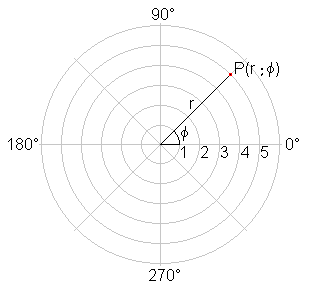
\includegraphics[width=3cm]{../FuVar/images/Ebene_polarkoordinaten.png}
    \end{minipage}&
	\begin{minipage}{3cm}
    	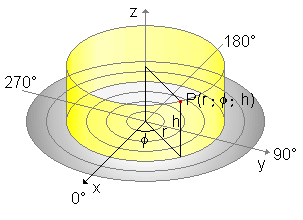
\includegraphics[width=4.2cm]{../FuVar/images/Zylinderkoordinaten.png}
    \end{minipage}&
	\begin{minipage}{3cm}
    	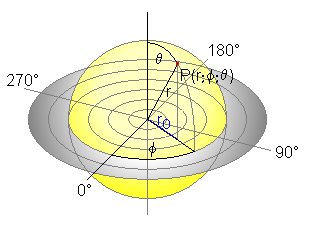
\includegraphics[width=5cm]{../FuVar/images/Kugelkoordinaten.png}
    \end{minipage}\\
	\hline
	Umrechnungs- formeln &
	\begin{minipage}{3cm}
    \vspace{0.1cm}
		$x=r\cos\varphi$\\
		$y=r\sin\varphi$    
    \vspace{0.1cm}
    \end{minipage}&	
	\begin{minipage}{4.2cm}
    \vspace{0.1cm}
    	$x=r\cos\varphi$\\
    	$y=r\sin\varphi$\\
    	$z=z$
    \vspace{0.1cm}
    \end{minipage}&	
	\begin{minipage}{7.5cm}
    \vspace{0.1cm}
    	$x=r\sin\vartheta\cos\varphi$\\
    	$y=r\sin\vartheta\sin\varphi$\\
    	$z=r\sin\vartheta$
    \vspace{0.1cm}
    \end{minipage}\\
	\hline
	Jacobi-Matrix $Df$ &
	\begin{minipage}{3cm}
    \vspace{0.1cm}
		$\begin{pmatrix}
         	\cos\varphi & -r\sin\varphi\\
         	\sin\varphi & r\cos\varphi
         \end{pmatrix}$
    \vspace{0.1cm}
    \end{minipage}&	
	\begin{minipage}{4.2cm}
    \vspace{0.1cm}
		$\begin{pmatrix}
         	\cos\varphi & -r\sin\varphi & 0\\
         	\sin\varphi & r\cos\varphi & 0\\
         	0 & 0 & 1
         \end{pmatrix}$
    \vspace{0.1cm}
    \end{minipage}&	
	\begin{minipage}{7.5cm}
    \vspace{0.1cm}
		$\begin{pmatrix}
         	\sin\vartheta\cos\varphi & -r\sin\vartheta\sin\varphi &
         	r\cos\vartheta\cos\varphi\\
         	\sin\vartheta\sin\varphi & r\sin\vartheta\cos\varphi &
         	r\cos\vartheta\sin\varphi\\
         	\cos\vartheta & 0 & -r\sin\vartheta
         \end{pmatrix}$
    \vspace{0.1cm}
    \end{minipage}\\
	\hline
	\begin{minipage}{2.5cm}
    	\vspace{0.1cm}
  		$detDf$   
  		\vspace{0.1cm}
    \end{minipage}&
		$r$ &
		$r$ &
		$r^2\cos\vartheta$\\
	\hline	
\end{tabular}
    


